\documentclass[twocolumn]{article}

\usepackage{abstract}
\usepackage{tabularx}

\usepackage{graphicx}
\graphicspath{ {Graphics/} }

\begin{document}

\title{Measurement of Mixed Species Ion Chain Temperature Using Spontaneous Reordering}
\author{John Wright \and Richard Graham \and Tomasz Sacrejda \and Zichao Zhou \and B.B. Blinov}
\date{\today}

\twocolumn[
\maketitle
\begin{onecolabstract}
	Quantum information processing with trapped ions often requires characterizing their motional heating rate so that this channel can be used to implement gates between arbitrary ions in the same trap.  We use the spontaneous reordering of \(Ba^+\) and \(Yb^+\) ions to estimate their temperature by comparison to a classical, numerical simulation.  This technique is easy to implement, and gives information about the motional coupling between Barium and Ytterbium as well as the average temperature and heating rate of the chain.
\end{onecolabstract}
]

	Trapped ions present an isolated quantum system that can be used to implement quantum algorithms.  Most proposals for transferring quantum information between ions rely on the motional degrees of freedom of the trap to couple distant ions.  Usually, phonons are exchanged between trapped ions to control the driven excitation of motional sidebands of electronic transitions [citation needed].  These proposals usually require ions to be cooled to the Lamb-Dicke limit or below and have a motional heating rate slow compared to the operation.  Most scalable ion trap quantum computer proposals utilize large number of ions per chain and surface electrode traps that significantly increase the trap heating rate and necessitate its measurement for different trap configurations.

	For this reason, many techniques to measure or estimate the heating rate of an ion chain have been developed.  The temperature can be measured directly using a narrow laser to compare the red and blue motional sideband strengths [citation needed].  Monitoring the flourescence rate of ions undergoing doppler recooling after heating can provide an estimate of the initial temperature that has been shown to compare well with direct measurements [citation needed].

	We trap \(^{138}Ba^+\) and \(Yb^+\) ions in a standard linear Paul trap.  The Barium ions are laser cooled and detected using a 493nm ECDL and a 650nm ECDL repump.  Ytterbium ions of unknown isotope are loaded by charge exchange with Barium ions and are not addressed by any lasers.  They are cooled by sympathetic cooling with the Doppler cold Barium ions.  An EMCCD camera with a wide field of view images the 493nm flourescence of the Barium ions, and the positions of the Ytterbium ions can be inferred from a series of images where the ions exchange positions.  We investigate whether the information from such a series of images can be used to estimate the average temperature of the chain.

\begin{figure}[ht!]
	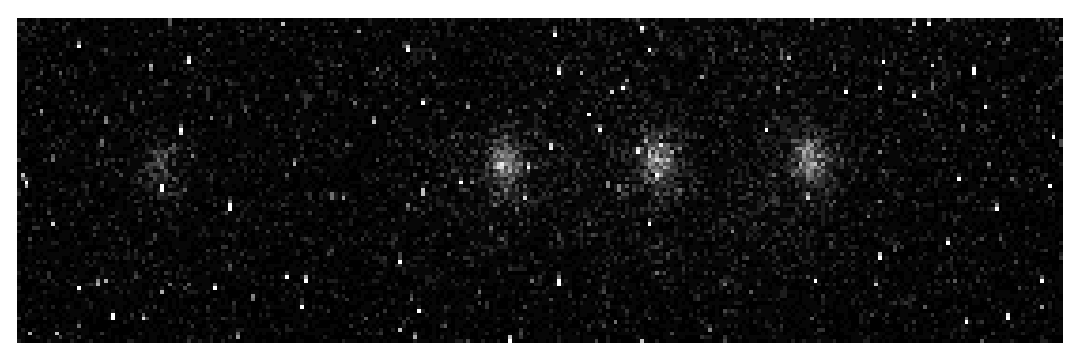
\includegraphics[width=0.48\textwidth]{example_data_7_3}
	\caption{Typical data from a chain of 4 \(^{138}Ba^+\) ions and 3 \(Yb^+\) ions.  The beam profile of the 493nm laser causes the outermost ions to be dimmer than the rest.}
\end{figure}

	Beginning with a trapped Doppler cold chain of \(Ba^+\) and \(Yb^+\), the 650nm repump laser is mechanically shuttered and the chain left in the dark for varying periods of time.  The lifetime of the repumped \(5D_{3/2}\) state is longer than any experimental dark time, so the 493nm laser has no effect.  The ions are heated from pseudopotential gradients, surface effects, and anomalous ion heating [citation needed].  The mechanical shutter is deactivated and the camera images the ions after the cooling lasers have recrystalized them.  The Barium ion positions in the images are tracked by an automatic-thresholding computer algorithm and the number of reordering events is recorded.  The onset of spontaneous reordering is relatively sharp in temperature, but is broadened in some of the data because the images can only be distinguished when ions of different species reorder.

	In order to estimate temperature from the collected data, a similar procedure is simulated using classical approximations and a numerical differential equation integrator.  A chain of mixed species ions is artificially cooled to the bottom of the trap.  The cooling is then removed and the ions are given a randomly directed initial velocity, corresponding to some initial temperature.  The ions are simulated for several hundred multiples of the trap frequency and then recooled by simulated Doppler cooling.  Finally the determination of reordering is made physically realistic by requiring that it involves different ion species.  The collected data is fit to the simulation using the initial temperature and heating rate of each chain as free parameters. Although the heating of the ion chain is handled unphysically, the separation of time scales between the heating rate and the trap frequency means that only the highest temperature the ions achieve is likely to cause reordering.  The qualitative features of the simulated data agree well with the experimental results.

\begin{figure}[ht!]
	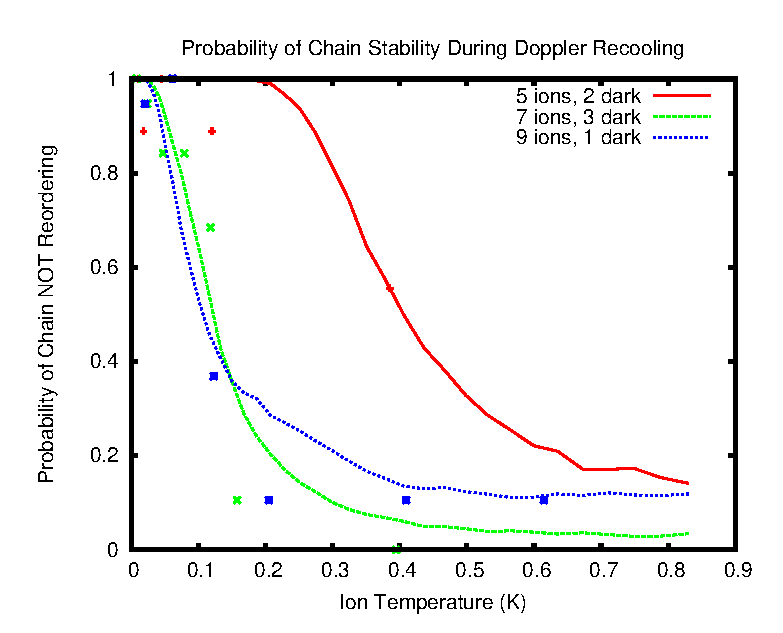
\includegraphics[width=0.48\textwidth]{results}
	\caption{Probability of ion chain stability during doppler recooling for 9 ions - 1 dark (green), 7 ions - 3 dark (blue), and 5 ions - 2 dark (red).  Points respresent actual data fit, curves respresent the results of described simulations.  Initial temperature and heating rate fit per chain.}
\end{figure}

	The initial temperature and heating rate for each configuration is given below:

\begin{tabularx}{\linewidth}{lll}
	Chain Description & Initial Temperature (K) & Heating Rate (K/s) \\
	\hline
	9 ions - 1 dark & 3 & 4 \\
\end{tabularx}

	

\end{document}

